\documentclass[a4paper]{article}
\usepackage{preamble}

% Setup title
\title{PHYSICS 2 - TERM 2}
\author{Marc Sanchis}
\date{April 2024 - June 2024}

\begin{document}

% Title
\newgeometry{top=2cm, bottom=5.5cm}
\maketitle

% Table of Contents
\renewcommand{\contentsname}{}
\tableofcontents

% Body
\newpage
\restoregeometry
\pagestyle{fancy}
\setcounter{section}{4}

\newcounter{ex}[section]
\newcounter{prob}[section]
\setcounter{ex}{0}
\setcounter{prob}{0}

\section{Magnetism in Matter}

\subsection{Magnetic Behaviour}
Materials fall into three groups based on their magnetic behaviour:

\begin{itemize}
    \item \textbf{Diamagnetic}: It has a weak, opposite-direction reaction to a $B$ field.
    \item \textbf{Paramagnetic}: With no $B$ their electrons have a defined magnetic moment, and when a magnetic field is applied, they have a slight attraction towards it.
    \item \textbf{Ferromagnetic}: Same as Paramagnetic, but its dipoles are aligned even before the $B$ the field is applied and has a very strong, attractive reaction.
\end{itemize}

For $B_{0}=0$, the vacuum has $(\vec{m}=\vec{0}, \vec{B}=\vec{0})$, Diamagnetic $(\vec{m}_{atomic}=\vec{0}, \vec{m}=\vec{0},\vec{B}=\vec{0})$, Paramagnetic $(\vec{m}_{atomic}\neq \vec{0},\vec{m}=\vec{0}\vec{B}=\vec{0})$, Ferromagnetic $(\vec{m}_{atomic}\neq\vec{0},\vec{m}\neq\vec{0}),\hspace{1ex}\vec{0}\in D:\sum\vec{m}$ .

For $B_{0}\neq 0$, the vacuum has $\vec{B}_{total}=\vec{B}_{0}$, Diamagnetic $\vec{B}_{total}<\vec{B}_{0}$, Paramagnetic $\vec{B}_{total}>\vec{B}_{0}$, Ferromagnetic $\vec{B}_{total}\gg \vec{B}_{0}$ .

\begin{align}
\vec{M}=\frac{d\vec{m}}{dv},\hspace{4ex}J_{S}&=|\vec{M}|,\hspace{4ex}dm=dI\cdot dS \\
\vec{B}_{total}&=\vec{B}_{0}+\vec{B}_{JS}
\end{align}

\note{If the magnetisation $M$ is constant, amperian bound currents appear in the material surface}
\begin{figure}[h]
    \centering
    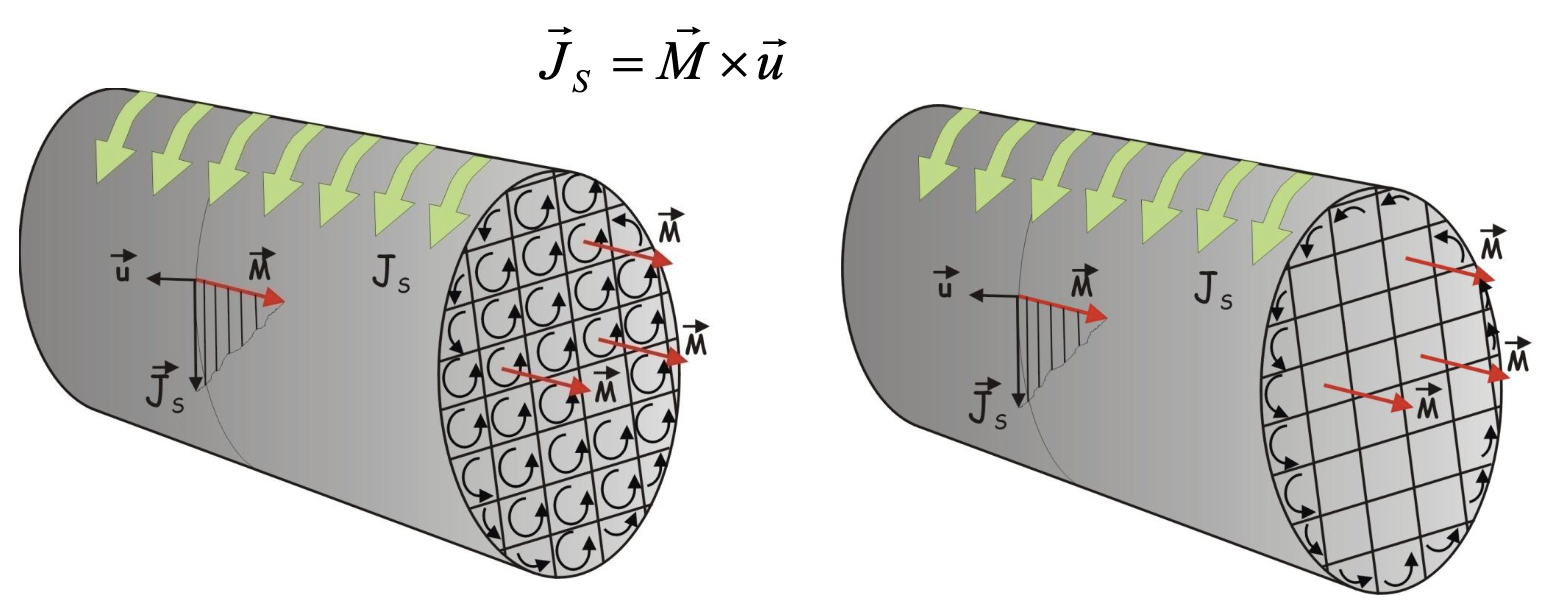
\includegraphics[width=0.5\textwidth]{IMG/js.png}
    \caption{Amperian bound currents appearing}
    \label{fig:js}
\end{figure}

\subsection{Magnetic Excitation}
\subsubsection{The H field}
The $H$ field only depends on the free current.
$$
\vec{H}=\frac{\vec{B}}{\mu_{0}}-\vec{M}, \hspace{4ex}\vec{B}=\mu_{0}(\vec{H}+\vec{M})\to B^*=\mu_{0} (H+M)
$$
$H$ can be demonstrated in two equivalent ways:
$$
\begin{cases}
&\oint \vec{H}\cdot d\vec{l}=\int_{C} \frac{\vec{B}}{\mu_{0}} \, d\vec{l}\,-\int_{C}^{} \vec{M} \, d\vec{l}\, = \frac{1}{\mu_{0}}[\mu_{0}nlI+\mu_{0}J_{S}l]-J_{S}l=nlI \\
&\oint_{C} \vec{H}\cdot d\vec{l}=Hl
\end{cases} \hspace{1ex}\to \boxed{H=nI}
$$
and
$$
\to\begin{cases}
B=\mu_{0}[nI+J_{S}]=\mu_{0}[nI+M] \\
B^*=\mu_{0}(H+M)
\end{cases}\hspace{1ex}\to \boxed{H=nI}
$$

\subsubsection{Ampère's Theorem for H}
Per Ampère's theorem for $H$:
$$
\oint_{C}\vec{H}\cdot d\vec{l}=I_{f r e e}, \hspace{4ex}Curl(\vec{H})=\vec{J}_{f r e e}
$$

\subsubsection{M-H Relationship}
The relationship between $M$ and $H$ is
$$
\vec{M}=\chi \vec{H}
$$
For diamagnetic materials $0<\chi\ll-1$, paramagnetic $0>\chi\ll 1$, ferromagnetic $1000<\chi<8000$.

$$
\vec{H}=\frac{\vec{B}}{\mu_{0}}-\vec{M}=\frac{\vec{B}}{\mu_{0}}-\chi \vec{H} \to \vec{B}=\mu_{0}(1+\chi)\vec{H}=\mu \vec{H}
$$
$$
\mu_{r}=\frac{\mu}{\mu_{0}}=1+\chi
$$

\stepcounter{prob}\vspace{2ex}\textbf{\textit{Prob.\thesection.\theprob: }}PB.6 Cylindrical tube of radius $r_{1},\,r_{2}$ and a charged conductive wire through the inside.
$$r_{1}=4mm,\,r_{2}=6mm,\,\chi=3\times 10^{-4},\,A=0,5A$$

$\triangleright$ a) Equivalent currents for the walls
\begin{align}
\oint\vec{H}d\vec{l}=I\implies \vec{M}&=\lambda \vec{H}\implies \vec{J}_{S}=\vec{M}\times \vec{u} \\
\text{Ampère's T. }\to Hl&=I\implies H =\frac{I}{2\pi r} \\
\end{align}
$$
\begin{cases}
M=0, & r<a,\,r>b \\
M=\chi \frac{I}{2\pi r}, & a<r<b\implies\vec{J}_{s}=\vec{M}\times \vec{u}\begin{cases}
r=r_{1}&\implies J_{Sr_{1}}=\chi \frac{I}{2\pi r_{1}} \\
r=r_{2}&\implies J_{Sr_{2}}=\chi \frac{I}{2\pi r_{2}}
\end{cases}
\end{cases}
$$
\begin{align}
J_{Sr_{1}}=3\times 10^{-4} \frac{0'5}{2\pi\, 4\times 10^{-3}}=\boxed{5'96\times 10^{-3}A / m} \\
J_{Sr_{2}} = 3\times 10^{-4} \frac{0'5}{2\pi\,6\times 10^{-3}}=\boxed{3'98 \times 10^{-3} A / m}
\end{align}
$\triangleright$ b) $B(r)$ for $b<r<c,\,r>c$
\begin{align}
\vec{B}=\mu \vec{H}=\mu _{r}\mu_{o}\vec{H} & =\mu_{o}(\chi+1)\vec{H}
\end{align}
$$
\begin{cases}
b<r<c,&B_{1}=\mu_{o}(\chi H) \frac{I}{2\pi r} \\
r>c,&B_{2}=\mu_{o}H
\end{cases}
$$
\begin{align}
B_{1}&=4\pi \times 10^{-7}(3\times 10^{-4}+1) \frac{0'5}{2\pi r}=\boxed{\frac{10^{-7}}{r}\,T} \\
B_{2}&=4\pi \times 10^{-7} \frac{0'5}{2\pi r}=\boxed{\frac{10^{-7}}{r}\,T}
\end{align}
\subsection{Ferromagnetism}
\setcounter{equation}{0}
A ferromagnetic material has the property $\mu\gg$ and by \textit{Ampère's Theorem} on a coiled toroid
$$
\oint_{C}\vec{H}d\vec{l}=I\implies H_{2}\pi r=NI\implies \boxed{H=\frac{NI}{2\pi r}}
$$
so we can see $H$ is linear with $I$, but $H$ is not linear with $B$ and $M$, because $\mu \neq \text{const}$, the curve describing this relation is the \textit{First Magnetisation Curve}.
$$
H\propto I,\hspace{4ex}\mu=B / H\implies 
$$

\begin{figure}[H]
    \centering
    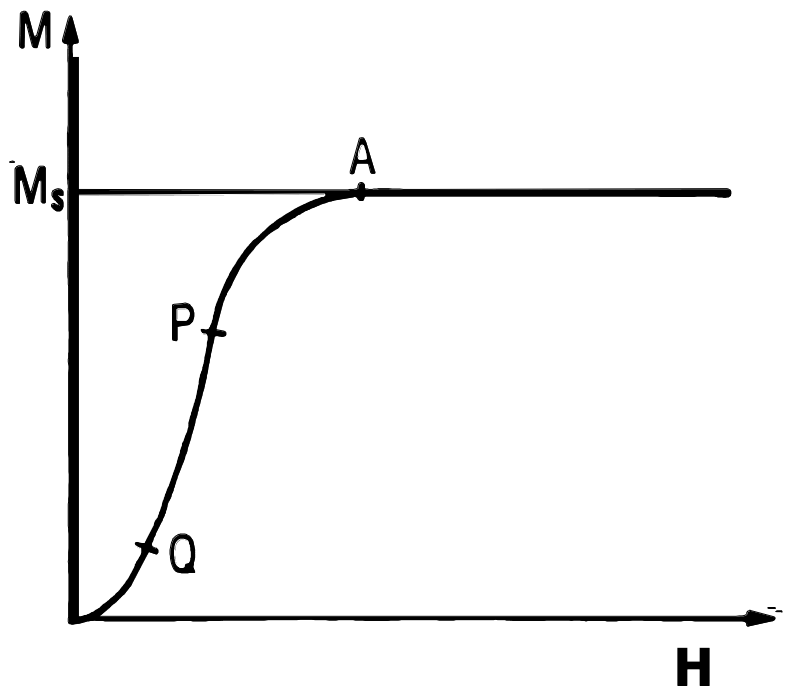
\includegraphics[width=0.33\textwidth]{IMG/mag_curve.png}
    \caption{Magnetisation curve}
    \label{fig:mag_curve}
\end{figure}

For any case different from the first excitation will not go through $M\cap H=0$, this is called the \textit{Hysteresis Cycle}.

\begin{figure}[H]
    \centering
    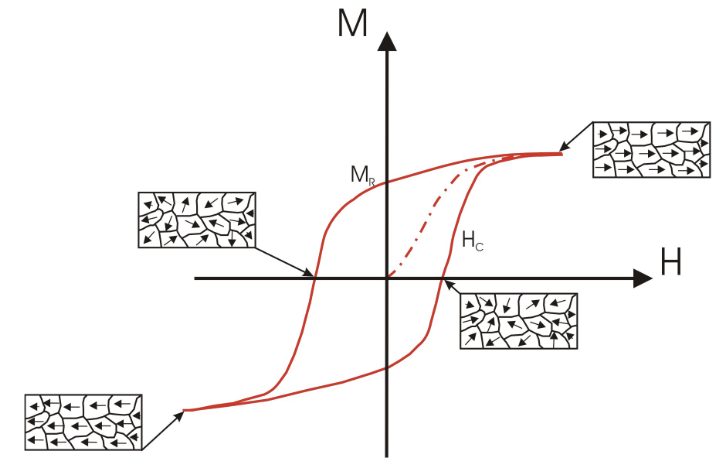
\includegraphics[width=0.33\textwidth]{IMG/hyst_cycle.png}
    \caption{Hysteresis cycle}
    \label{fig:hyst_cycle}
\end{figure}

A ferromagnetic material can be returned to its initial state by using constantly smaller secondary hysteresis cycles.

\subsection{Permanent Magnets}
\setcounter{equation}{0}
A magnetic cylinder can be calculated like a solenoid and vice versa, as $n=J_{S}=M$
\begin{align*}
&\text{Solenoid }\to & B&=\frac{\mu_{o}nI}{2}(\sin \phi_{2}-\sin \phi_{1}) \\
& \text{Cylinder }\to & B&=\frac{\mu _{o}J_{S}}{2}(\sin \phi_{2}-\sin \phi_{1})=\frac{\mu_{o}M}{2}(\sin \phi_{2}-\sin \phi_{1})
\end{align*}
this way $H$ can be obtained on the inside
\begin{align*}
H_{\text{in}}&=\frac{\mu_{o}M}{2\mu_{o}}(\sin \phi_{2}-\sin \phi_{1})-M= \\
&=\frac{H}{2}((\sin \phi_{2}-\sin \phi_{1})-2)<0
\end{align*}
so $H$ runs in the opposite way inside the magnet to let $M$ manifest, nevertheless, on the outside $\vec{H}\parallel \vec{B}$ 
$$
H_{\text{out}}=\frac{M}{2}(\sin \phi_{2}-\sin \phi_{1})
$$
\stepcounter{ex}\vspace{2ex}\textbf{\textit{Ex.\thesection.\theex: }}PB.8 A permanent magnet with a ring form with a gap $e=2mm$ and a medium radius $r=10cm$, the magnetic field in the gap is $B=0'02T$.

$\triangleright$ a) Magnetic excitation inside the magnet
\begin{align}
\text{Ampère's T. }\to \oint_{C}\vec{H}d\vec{l}=I_{\text{inter}} =0
\end{align}
\vspace{1ex}\note{$H$ is not null, as the magnet has magnetisation of its own, while the currents are non-existent}\vspace{1ex}

\begin{align}
H_{\text{Fe}}&=H_{e} \frac{e}{l_{\text{Fe}}}=\frac{B_{e}}{\mu_{o}} \frac{e}{2\pi r-e} \\
&=-15915'49\cdot \frac{2\times 10^{-3}}{(2\pi \cdot 10\times 10^{-2}-2\times 10^{-3})} \\
&=\boxed{-50'8 A / m}
\end{align}

$\triangleright$ b) Magnetisation of the magnet

The field in the gap is the same as the field of the magnet; the flux can prove this
\begin{align}
\phi=\int \vec{B}d\vec{S}\, =B_{\text{Fe}}S_{\text{Fe}}=B_{e}F_{e}\implies B_{\text{Fe}}=B_{e}
\end{align}

For the magnetisation, we can use the excitation formula
\begin{align}
\vec{H}_{\text{Fe}}&=\frac{\vec{B}_{e}}{\mu_{o}}-\vec{M} =\frac{0'02}{4\pi \times 10^{-7}}-\vec{M}=-50'8 \\
M&=\frac{0'02}{4\pi \times 10^{-7}} -H=\boxed{1'6\times 10^{4}A / m}
\end{align}
\subsubsection{Ampère's Theorem With the Flux Prove of Gap-Magnet Magnetic Equality}
\setcounter{equation}{0}
If we divide the gapped magnet into four sections, we get
\begin{align}
\oint_{C}\vec{H}d\vec{l}=I\implies H_{1}l_{1}+H_{2}l_{2}+H_{3}l_{3}+H_{4}l_{4}+H_{e}l_{e}
\end{align}
therefore either $I$ or $B$ and $\mu_{1},\,\mu_{2},\,\mu_{3},\,\mu_{4}$ must be known. If only $B_{e}$ and the $\mu$ of the sections, we can prove the \textit{gap-magnet magnetic field equality}
\begin{align}
\phi=\int _{S}\vec{B} \, d\vec{S}\, &\implies B_{1}S=B_{2}S=B_{3}S=B_{4}S=B_{e}S \\
&\implies B_{1}=B_{2}=B_{3}=B_{4}=B_{e} 
\end{align}
\subsection{Magnetic Circuits}
\setcounter{equation}{0}
A magnetic circuit includes a ferromagnetic material with a magnetic field induced by a current; it transforms electricity in magnetisation.

\begin{figure}[H]
    \centering
    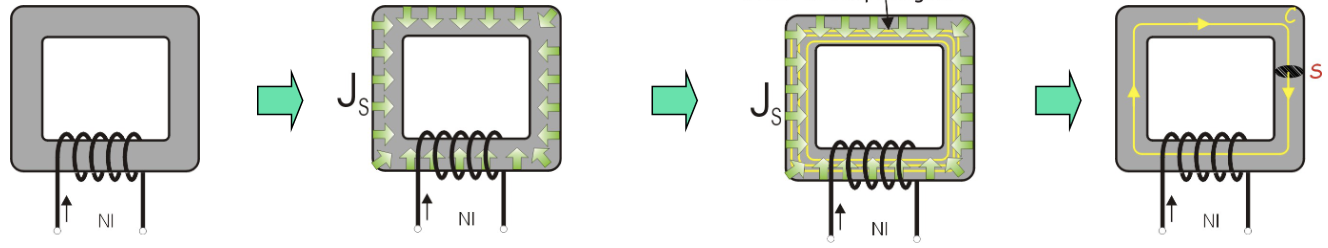
\includegraphics[width=\textwidth]{IMG/mag_circuit.png}
    \caption{Caption}
    \label{fig:enter-label}
\end{figure}

\subsubsection{Hopkinson's Law}
\setcounter{equation}{0}
By adapting \textit{Ampère's Theorem}, we get a new law that rules magnetic circuits
$$
\oint_{C}\vec{H}d\vec{l}=\oint_{C}Hdl=\oint_{C}\frac{B}{\mu}dl=\oint \frac{\phi}{\mu S}dl=\phi \oint \frac{dl}{\mu S}=\phi \cdot R=NI
$$
$$
\text{Hopkinson's Law}\to \boxed{\phi \cdot R=NI=F}
$$

\setcounter{equation}{0}
\stepcounter{prob}\vspace{2ex}\textbf{\textit{Prob.\thesection.\theprob: }}PB.12 Closed ring $r=0'2m,\,S=1\times10^{-4}m^{2},\,\mu_{r}=1000,\,N=500,\, I=2A$

$\triangleright$ a) Magnetic Excitation
\begin{align}
&\begin{cases}
\oint_{C}=\vec{H}d\vec{l}=I_{\text{inter}}=NI \\
C=\oint_{C}Hdl\cos 0=H\oint_{C}dl=H2\pi r
\end{cases}\implies  \\
\implies H&=\frac{NI}{2\pi r}=\frac{500\cdot 2}{2\pi \cdot20\times 10\times^{-2}}=\boxed{795'7\,A /m}
\end{align}
$\triangleright$ b) Magnetic Field
\begin{align}
B=\mu H=\mu_{r}\mu_{o}H=1000\cdot4\pi \cdot 795'7=1\,T
\end{align}

$\triangleright$ c) Reluctance of the circuit
\begin{align}
R&=\frac{l}{\mu S}=\frac{2\pi r}{\mu_{r}\mu_{o}S}= \\
&=\frac{2\pi \cdot 20\cdot 10^{-2}}{1000\cdot 4\pi \times 10^{-7}\cdot 10\times 10^{-4}}=\boxed{10^{6}\, H^{-1}}
\end{align}

$\triangleright$ d) Magnetic flux
\begin{align}
\phi&=\int _{S} \vec{B}\,d\vec{S}=\int _{S}B\,dS\cos_{0}\, = \\
&=1\cdot 10 \times 10^{-4}=\boxed{ 1\, mWb}
\end{align}
$\triangleright$ e) Auto-induction Index
\begin{align}
L&=\frac{\mu_{\text{total}}}{I}=\frac{\mu N}{I}=\frac{1000\cdot 500}{2}=\boxed{0'25\,H}
\end{align}

A $2mm$ gap is created, maintaining the magnetic permeability.

$\triangleright$ f) New Reluctance
\begin{align}
\oint_{C}\vec{H}d\vec{l}&=I\implies H_{\text{Fe}}\,l_{\text{Fe}}+H_{e}\,l_{e}=NI \\
\phi&=B_{\text{Fe}}\, S_{\text{Fe}}=B_{e}\,S_{e} \implies B_{\text{Fe}}=B_{e} \implies \\
\implies&\mu H_{\text{Fe}}=\mu_{o}H_{e}\implies H_{e}=\frac{\mu_{o}\mu_{r}}{\mu_{o}}H_{\text{Fe}}=1000H_{\text{Fe}} \\
&\begin{cases}
H_{\text{Fe}}\,l_{\text{Fe}}+H_{e}\,l_{e}=NI \\
H_{e}=1000H_{\text{Fe}}
\end{cases}
\end{align}
\begin{align}
R'&=R_{\text{Fe}}+R_{e}=\frac{l-e}{\mu_{r}\mu_{o}S}+\frac{e}{\mu _{o}S}=\boxed{2589957'88\,H^{-1}}
\end{align}

$\triangleright$ g) New Flux
\begin{align}
\phi '=\frac{NI}{R_{eq}}=\boxed{3'87\times 10^{-4}\,Wb}
\end{align}

$\triangleright$ h) New Magnetic Field
\begin{align}
B'=\frac{\phi'}{S}=\boxed{0'387\,T}
\end{align}

\stepcounter{prob}\vspace{2ex}\textbf{\textit{Prob.\thesection.\theprob: }}PB.13 A circuit with two $5\times 10^{-4}m$ gaps, $S=50cm^{2},\,l=0'98m,\,\mu=400\mu_{o},\,N=1000$ 

$\triangleright$ a) The intensity for $B=0,6\,T$
\begin{align}
\text{Hopkinson}\to NI&=R_{eq}\phi \\
I&=\frac{R_{eq}\phi}{N} \\
\phi&=B_{\text{Fe}}\,S_{\text{Fe}}=B_{e}\,S_{e} & S_{\text{Fe}}=S_{e}\implies B_{\text{Fe}}=B_{e}=0'6\,T \\
&=0'6\cdot 50\times 10^{-4}=3\,mWb \\
&\begin{cases}
\phi=3\times 10^{-3}
\end{cases}
\end{align}
\begin{align}
R_{eq}&=R_{\text{Fe}}+2R_{e}=\frac{l_{\text{Fe}}}{\mu_{r}\mu_{o}S}+2 \frac{e}{\mu_{o}S}=\frac{1}{\mu_{o}S}\left[ \frac{l_{\text{Fe}}}{\mu_{r}}+2e \right]= \\
&=\frac{1}{4\pi \times 10^{-7}\cdot 50\times 10^{-4}}\left[ \frac{98\times 10^{-2}}{400}+2\cdot 0'5\times 10^{-2} \right]= \\
&=1981479'05\,H^{-1} \\
&\begin{cases}
\phi=3 \times 10^{-3} \\
R_{eq}=1981479'05
\end{cases}
\end{align}
\begin{align}
I=\frac{R_{eq}\phi}{N}=\boxed{5'9\,A}
\end{align}

$\triangleright$ b) Magnetic Excitation between metal and gap
\begin{align}
B_{\text{Fe}}&=B_{e}\implies \mu_{r}\mu_{o}H_{\text{Fe}}=\mu_{o}H_{e}\implies H_{\text{Fe}}=\frac{H_{e}}{\mu_{r}} \\
H_{\text{Fe}}&=\frac{H_{e}}{400}=\boxed{1193'7\,A / m}
\end{align}

$\triangleright$ c) Auto-induction Index
\begin{align}
L&=\frac{N^{2}}{R_{eq}}=\frac{1000^{2}}{1981479'05}=\boxed{0'504\,H}
\end{align}

\textbf{\textit{PB.7}}

\setcounter{equation}{0}
\stepcounter{prob}\vspace{2ex}\textbf{\textit{Prob.\thesection.\theprob: }}PB.7 Two parallel conductors of infinite length on the $XY$ plane are $16cm$ away from each other and are equally distanced from the centre $(0,0,0)$. Both are charged with $5A$ and the exterior is a magnetic material of permeability $\mu_{r}=500$. The point $P$'s coordinates are $(0,8,0)$.

\begin{figure}[H]
    \centering
    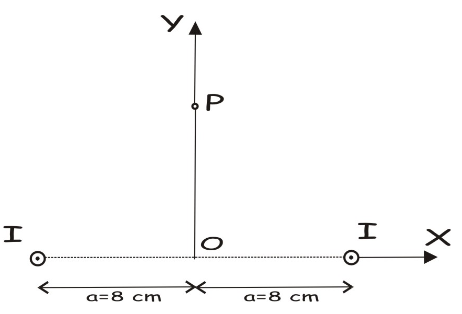
\includegraphics[width=0.33\textwidth]{IMG/pb7.png}
    \caption{Exercise 7}
    \label{fig:pb7}
\end{figure}

I will be calling the conductors $1,\,2$ from $-x$ to $+x$.

$\triangleright$ a) Magnetic Excitation at point $P$
\begin{align}
\overline{IP}&=\sqrt{ 8^{2}+8^{2} }\approx 11'3137cm=0'113137m \\
\oint_{C}\vec{H}d\vec{l}&=NI\implies H\oint dl\cdot \cos 0=I\implies H=\frac{I}{2\pi r} \\
H_{P}&=-H_{1x}+H_{1y}-H_{2x}-H_{2y}=-H_{1x}-H_{2x}= \\
&=\langle H_{1x}=H_{2x} \rangle=2 \frac{5}{2\pi r}\cos 45=-\frac{5}{\pi r}\cos 45 \mathbf{i}
\end{align}
$$
\boxed{H_{P}\approx-9'947\mathbf{i}\,A / m}
$$

$\triangleright$ b) Magnetic field at P
\begin{align}
B=\mu H & =\mu_{o}\mu_{r}H=4\pi\times 10^{-7}\cdot 500\cdot (-9'947)\approx-0'00625
\end{align}
$$
\boxed{B_{P}=-6'25\Vec{\textbf{i}}\,mT}
$$

$\triangleright$ c) Flux at $O(0,0,0)$
\begin{align}
\Vec{B}_O=\Vec{B}_{1}+\Vec{B}_{2}
\end{align}
As the conductors' are at the same distance from $O$, the fields will cancel out like so
$$
\boxed{B_O=\Vec{0}\,T}
$$


\section{Maxwell's Equations}

\setcounter{equation}{0}
\subsection{Previous Concepts}
\setcounter{equation}{0}
The Nabla operator is described as
$$
\vec{\nabla}=\frac{\partial}{\partial x}\mathbf{i}+\frac{\partial}{\partial y}\mathbf{j}+\frac{\partial}{\partial z}\mathbf{k}
$$
now, a field can be scalar or vector. If Nabla acts on a \textit{scalar field} ($\vec{\nabla}\cdot f)$, it is called a \textbf{\textit{gradient}}; on a \textit{vector field} simple relation ($\vec{\nabla}\cdot\vec{f}$), it is called \textit{\textbf{divergence}}, and for a vector relation ($\vec{\nabla}\times \vec{f}$), \textit{\textbf{rotational}}.

\stepcounter{ex}\vspace{2ex}\textbf{\textit{Ex.\thesection.\theex: }}Calculate $\vec{\nabla}\vec{A}$ on point $P(1,-1,0)$ for $\vec{A}=x^{2}z\mathbf{i}-2y^{3}z^{2}\mathbf{j}+x^{2}y^{2}z\mathbf{k}$
\begin{align}
\text{div}\vec{A}=\vec{\nabla}\vec{A}&=\left(\frac{\partial}{\partial x}\mathbf{i}+\frac{\partial}{\partial y}\mathbf{j}+\frac{\partial}{\partial z}\mathbf{k}\right)\cdot [x^{2}z\mathbf{i}-2y^{3}z^{2}\mathbf{j}+x^{2}y^{2}z\mathbf{k}]= \\
&=\frac{\partial}{\partial x}(x^{2}z)+\frac{\partial}{\partial y}(2y^{3}z^{2})+\frac{\partial}{\partial z}(x^{2}y^{2}z)= \\
&=2xz+6y^{2}z^{2}+x^{2}y^{2}
\end{align}
$$
\Vec{\nabla}\Vec{A}=2xz+6y^{2}z^{2}+x^{2}y^{2},\,\forall(x,y,z)
$$
\begin{align}
[\vec{\nabla}\vec{A}]_{P}=2\cdot 1\cdot 0-6\cdot (-1)^{2}\cdot 0+1^{2}\cdot (-1)^{2}=\boxed{1}
\end{align}

\stepcounter{ex}\vspace{2ex}\textbf{\textit{Ex.\thesection.\theex: }}Calculate $\vec{\nabla}\times \vec{A}$ on point $P(1,-1,1)$ for $\vec{A}=xz^{3}\mathbf{i}-2x^{2}yz\mathbf{j}+2yz^{4}\mathbf{k}$
\begin{align}
\text{rot}\vec{A}=\vec{\nabla}\times \vec{A}&=\begin{array}{|ccc|}
\mathbf{i} & \mathbf{j} & \mathbf{k} \\
\frac{\partial}{\partial x} & \frac{\partial}{\partial y} & \frac{\partial}{\partial z} \\
A_{x} & A_{y} & A_{z}
\end{array}= \\
&=\frac{\partial A_{z}}{\partial y}\mathbf{i}+\frac{\partial A_{x}}{\partial z}\mathbf{j}+\frac{\partial A_{y}}{\partial x}\mathbf{k}-\frac{\partial A_{x}}{\partial y}\mathbf{k}-\frac{\partial A_{y}}{\partial z}\mathbf{i}-\frac{\partial A_{z}}{\partial x}\mathbf{j}= \\
&=2xyz+3xz^2+y^3z^2-xz^3-4y^3z-2xy^2
\end{align}

The Laplacian is the squared of a Nabla operator
$$
\Delta=\vec{\nabla}\cdot \vec{\nabla}=\vec{\nabla}^{2}=\frac{\partial^{2}}{\partial x^{2}}+\frac{\partial^{2}}{\partial y^{2}}+\frac{\partial^{2}}{\partial z^{2}}
$$

\setcounter{equation}{0}
\subsection{Divergence Theorem}
\setcounter{equation}{0}
The divergence measures the field generation in a volume
$$
\vec{\nabla}\vec{E}=\lim_{ \Delta V \to 0 } \left[ \frac{1}{\Delta V}\iint_{\Delta S}\vec{E}\,d\vec{S} \right]=\frac{d\Phi}{dV}
$$

\begin{figure}[H]
    \centering
    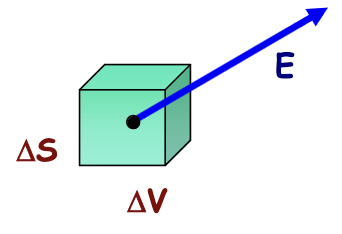
\includegraphics[width=0.33\textwidth]{IMG/div.png}
    \caption{Divergence representation}
    \label{fig:div}
\end{figure}

\subsubsection{Second Maxwell Equation}
\setcounter{equation}{0}
If we measure a field $\vec{B}$, there won't be any generator in it, so its divergence is null
$$
\boxed{\vec{\nabla}\vec{B}=0}
$$
and the flux through a closed section is also null
$$
\Phi=\int _{S_c} \vec{B}\,d\vec{S} \,=\int _{v} \vec{\nabla}\vec{B}\, dv\, =0
$$
it is logical to see that if $\vec{\nabla}\vec{f}=0$, then the field has a conservative flux, this is called a \textit{solenoidal} field. If $\vec{\nabla}\vec{f}\neq 0$, then the field is a generator, if positive, an emitter and, if negative, a receiver.

\stepcounter{ex}\vspace{2ex}\textbf{\textit{Ex.\thesection.\theex: }}Flux in the field 

$\triangleright$ a) $\vec{E}=x\mathbf{i}+y\mathbf{j}+z\mathbf{k}$ 
\begin{align}
\Phi&=\oint_{S}\vec{E}\,d\vec{S}=\int _{v}\vec{\nabla}\vec{E} \, dv\,  \\
\vec{\nabla}\vec{E}&=\left( \frac{\partial}{\partial x}+\frac{\partial}{\partial y}+\frac{\partial}{\partial z} \right)(x\mathbf{i}+y\mathbf{j}+z\mathbf{k})=3 \\
\Phi&=3\oint_{S}d\vec{S}=3a^{3}
\end{align}
$$
\boxed{\Phi=3a^{3}}
$$

$\triangleright$ b) Sphere $R=r$
\begin{align}
\Phi&=\oint_{S}\vec{E}\,d\vec{S}=\frac{q}{\varepsilon_{o}}= \\
&=\int _{v}\rho \, dv\, =\frac{\int _{v}\rho \, dv\, }{\varepsilon_{o}}
\end{align}
\subsubsection{First Maxwell Equation}
\setcounter{equation}{0}
\begin{align}
\begin{cases}
\Phi=\oint_{S}\vec{E}\,d\vec{S}=\int _{v}\vec{\nabla}\vec{E} \, dv\, \\
\Phi=\oint_{S}\vec{E}\,d\vec{S}=\int _{v}\rho \, dv\, =\frac{\int _{v}\rho \, dv\,}{\varepsilon_{o}}
\end{cases}\implies \boxed{\vec{\nabla}\vec{E}=\frac{\rho}{\varepsilon_{o}}}
\end{align}

\stepcounter{ex}\vspace{2ex}\textbf{\textit{Ex.\thesection.\theex: }}Let the vector field be $\vec{F}=x^{3}\mathbf{i}+y^{3}\mathbf{j}+xy\mathbf{k},\,P(X_{P},Y_{P},Z_{P})$ 

\begin{figure}[H]
    \centering
    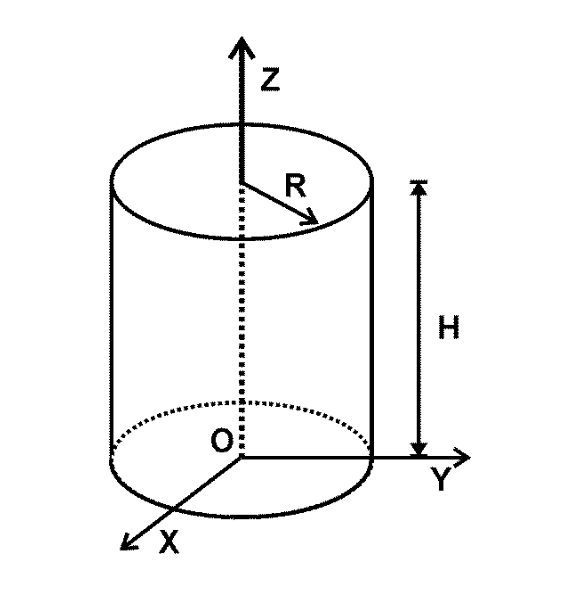
\includegraphics[width=0.25\textwidth]{IMG/c1_rec_2020.png}
    \caption{}
    \label{fig:c1_rec_2020}
\end{figure}

$\triangleright$ a) $[\text{rot}(\mathbf{F})]_{x}$ 
\begin{align}
[\vec{\nabla}\times \vec{F}]_{x}&=\begin{array}{|ccc|}
\mathbf{i} & \mathbf{j} & \mathbf{k} \\
\partial x & \partial y & \partial z \\
x^{3} & y^{3} & xy
\end{array}=\partial_{y}(xy)-\partial_{z}(y^{3})=x\mathbf{i}
\end{align}
$$
\boxed{[\vec{\nabla}\times \vec{F}]_{x_{P}}=X_{P}\,[V / m^{2}]}
$$

$\triangleright$ b) $\text{div}\mathbf{F}$
\begin{align}
\vec{\nabla}\vec{F}=\partial_{x}(x^{3})+\partial_{y}(y^{3})+\partial_{z}(xy)=3x^{2}+3y^{2}+0
\end{align}
$$
\boxed{[\vec{\nabla}\vec{F}]_{P}=3(X_{P}^{2}+Y_{P}^{2})\,[V / m^{2}]}
$$

$\triangleright$ c) Flux $\Phi_{\mathbf{F}}$ through the cylinder
\begin{align}
\Phi&=\int _{v}\vec{\nabla}\vec{F} \, dv\, =\int _{v}3(\overbrace{X_{P}^{2}+Y_{P}^{2}}^{r^{2}}) \, dv\,= \\
&& \implies(1)&=\iiint_{3}3(X_{P}^{2}+Y_{P}^{2})\,dx\,dy\,dz \\
&&\implies(2)&=\langle dv=dS\cdot h=2\pi rh\,dr\rangle = \\
&&&=\int_{0}^{R} 3r^{2}\cdot 2\pi rh \, dr\, = \\
&&&=6\pi h \frac{R^{4}}{4}=\boxed{\frac{3\pi r^{4}h}{2}\,[Vm]}
\end{align}

\subsection{Rotational Theorem}
\setcounter{equation}{0}
The rotational measures the circulation over surface unit
$$
\text{rot}\vec{A}\cdot d\vec{S}=\oint\vec{A}\,d\vec{l}=dC
$$
\subsubsection{Stokes' Theorem}
\setcounter{equation}{0}
\begin{align}
\text{rot}\vec{A}&=\frac{dC}{dS} &\Leftarrow \text{Stokes T. } \to C&=\oint_{C}\vec{A}\,d\vec{l}=\int _{S}(\vec{\nabla}\vec{A}) \, d\vec{S}\, 
\end{align}

\begin{figure}[H]
    \centering
    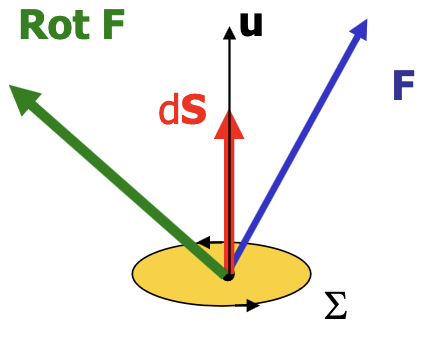
\includegraphics[width=0.33\textwidth]{IMG/rot.png}
    \caption{Rotational representation}
    \label{fig:rot}
\end{figure}

for a conservative field $\vec{\nabla}\times\vec{A}=0 \iff C=0$.

\stepcounter{ex}\vspace{2ex}\textbf{\textit{Ex.\thesection.\theex: }}Let the field be $\mathbf{F}=-y^{3}\mathbf{i}+x^{3}\mathbf{j}+z^{3}\mathbf{k}$

\begin{figure}[H]
    \centering
    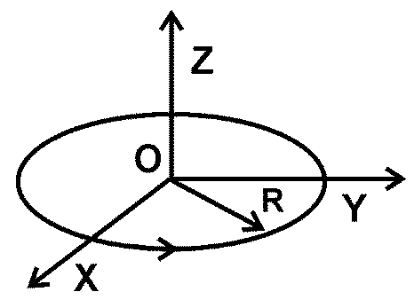
\includegraphics[width=0.33\textwidth]{IMG/c1_2020.png}
    \caption{}
    \label{fig:c1_2020}
\end{figure}

$\triangleright$ a)
\begin{align}
\vec{\nabla}\vec{F}
\end{align}

$\triangleright$ b)
\begin{align}
\vec{\nabla}\times \vec{F}&=\begin{array}{|ccc|} 
\mathbf{i} & \mathbf{j} & \mathbf{k} \\
\partial x & \partial y & \partial z \\
-y^{3} & x^{3} & z^{3}
\end{array} =\partial_{x}(x^{3})\mathbf{k}+\partial_{y}(y^{3})\mathbf{k}=\boxed{3(x^{3}+y^{3})\mathbf{k}}
\end{align}

$\triangleright$ c) Circulation $C_{\mathbf{F}}$ the circumference of $R=r$
\begin{align}
C&=\oint_{C}\vec{F}\,d\vec{l}=\int _{S}(\vec{\nabla}\times \vec{F}) \, d\vec{S}\,=\int_{0}^{R} 3r^{2}\cdot 2\pi r \, dr\,= \\
&=6\pi \frac{R^{4}}{4}=\boxed{\frac{3}{2}\pi r^{4} } 
\end{align}


\end{document}
